%\subsection{2. Prototype - Bus stop procedure}
%The second component is focused on detecting and performing a bus stop, and is built using the component of the steering object. 

%Using the requirements, this component needs to:\\
%    - Detect Bus Stops\\
%    - Stop parallel to the curb\\
%    - Stop within 1 cm of the curb

%The track will need to have some bus stops build on it, and it will also need to have some way to signal to the bus that a bus stop is coming up. This will most likely be a coloured piece of tape, that the bus will recognise with a LEGO colour sensor.\info{This is at least the plan as of this moment.}  Furthermore the track will also have to be circular to allow for the bus to keep driving around on the track and make repeated stops at the bus stops.



%\subsection{ Bus stop procedure \& Speed Controller}
%Intro: beskriv curb/bus stop procedure


%\textbf{Bus stop procedure} \newline

%\textbf{Speed Controller} \newline


%\textbf{Track requirements} \newline
%The redesigned track for the second iteration can be seen on figure.\todo{some stuff to fix here} %\ref{Track2Layout}.
%The track is quite similar to the first track, however in this iteration the track contains a bus stop, and it is a loop. Furthermore the aspect ratio have been changed slightly to fit the redesigned bus, that means the minimal turning radius and lane width have been recalculated as described in appendix \ref{laneCalculations}. Lastly the track contains three new tape colours placed between the two lane tapes. The three colours are to be used with the nxt color sensor to detect incoming bus stops, and to determine the speed limit of the road.

%The new requirements for the track is therefore as follows:
%\begin{itemize}
%  \item Detect Bus Stops
%  \item Stop parallel to the curb(tape)
%  \item Stop within 1 cm of the curb(tape)
%  \item Stop so the bus sign is 1cm from the right corner of the bus
%  \item Red tape to illustrate an incoming bus stop
%  \item Green tape to illustrate high speed zone(Major Highway)
%  \item Blue tape to illustrate low speed zone(Street)
%\end{itemize}

%\begin{figure}[H]
%    \label{Track2Layout}
 %   \centering
  %  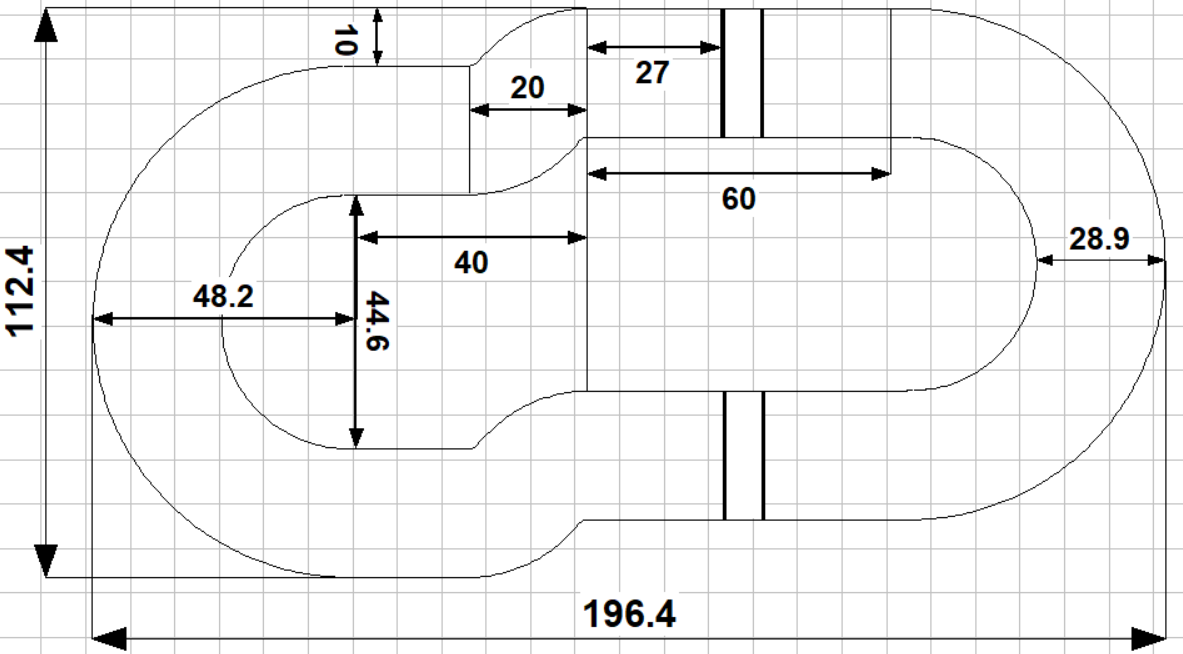
\includegraphics[width=0.8\textwidth]{Images/Tracks/Track1.PNG}
   % \caption{Track 2 Layout in cm}
%\end{figure}

%\textbf{Bus Reconstruction} \newline
%The redesigned bus can be seen on figure \ref{busDesign2}\todo{Missing picture of bus to reference}. The bus was redesigned to fix a couple of issues which was found upon testing in the first iteration.

%\begin{itemize}
 % \item Rear wheels felt off after the bus had driven for some time
  %\item Unbalanced weight, which made it hard for the bus to turn left, but not right.
  %\item The width and depth of the bus was not consistent, e.g. the ultrasonic sensor was placed too far in front. 

%\end{itemize}

%insert billede.












%OLD:
%As previously mentioned
%\ref{solvingRequirements
%\todo{fix}, we intend wish to detect a physical object emulating a sign and not just a drawing on the tracks. Towards this end we will be attempting to use a NXT CamV4 Sensor and some image recognition algorithm. 


%The bus scale should be a close approximate of a real bus scale as \cite{DriveingCurves}, 